\documentclass{bioinfo}
\copyrightyear{2015}
\pubyear{2015}

\begin{document}
\firstpage{1}

\title[VALET]{VALET: \emph{de novo} pipeline for finding metagenomic mis-assemblies}
\author[Hill \textit{et~al}]{Christopher Michael Hill\,$^{1,2,*}$, Jonathan Gluck\,$^{1}$, Victoria Cepeda\,$^{1,2}$, Matheiu Almedia\,$^{2}$, Sergey Koren\,$^{1,2}$, Atif Memon\,$^{1}$, and Mihai Pop\,$^{1,2}$\footnote{to whom correspondence should be addressed}}
\address{$^{1}$Department of Computer Science,
University of Maryland, College Park, Maryland, 20742
USA\\ $^{2}$ Center
for Bioinformatics and Computational Biology, University of
Maryland, College Park, Maryland, 20742 USA.}

\history{Received on XXXXX; revised on XXXXX; accepted on XXXXX}

\editor{Associate Editor: XXXXXXX}

\maketitle

\begin{abstract}

\section{Summary:}
%Metagenomic assembly is often more challenging than single genome assembly due to the presence of intrapopulational variations, greatly varying organism abundances, and conserved genomic regions between closely-related species.
Existing methods for detecting mis-assemblies rely on the existence of reference genomes, which are not always available.
Here, we present VALET, the first \emph{de novo} pipeline for detecting assembly erros in metagenomic assemblies.
VALET flags regions in the assembly containing inconsistencies between sequence generation process and the assembled region.
\section{Availability:}
https://github.com/cmhill/VALET
\section{Contact:} \href{cmhill@umiacs.umd.edu}{cmhill@umiacs.umd.edu}
\end{abstract}

\section{Introduction}
%Metagenomics is characterizing the environment around us.

Genome assembly of single organisms is made difficult due to the presence of sequencing errors and repeats.
This difficulty is compounded in metagenomic samples due to varying organism abundances, intrapopulational variations, and conserved genomic regions between closely-related species.
Since many downstream applications rely on metagenome assemblies, it is critical that the assembly is error-free.
Existing methods for finding mis-assemblies primarily focus on single genome assemblies and fall into two categories: reference-based and \emph{de novo} evaluation.

Reference-based methods use a collection of, often manually curated, reference genomes, while \emph{de novo} methods look for inconsistencies between characteristics of the data generation process and the resulting assembly.
QUAST~\citep{gurevich2013quast} is a reference based method that identifies mis-assemblies and structural variants in an assembly relative to a user provided reference genome.
QUAST leverages existing methods (Plantagora~\citep{barthelson2011plantagora},
GeneMark.hmm~\citep{lukashin1998genemark}, GlimmerHMM~\citep{majoros2004tigrscan}) and quality metrics (GAGE~\citep{salzberg2011gage}).
Though QUAT is able to calculate a number of quality metrics, such as __ADD Examples__, without a reference genome, these metrics only provide information about the overall quality of the assembly not assembly accuracy.
% QUAST uses the Plantagora’s definition of a mis-assembly,
% i.e., a mis-assembly breakpoint is defined as a position in the assembled contigs where (1) the left flanking
% sequence aligns over 1kb away from right flanking sequence on the reference, or (2) the sequences overlap by
% over 1kb, or (3) the right flanking sequence aligns on opposite strands or different chromosomes.

\emph{De novo} techniques for detecting mis-assemblies in single genomes rely on looking for inconsistencies between the sequence generation process and the resulting assembly.
In other words, given a model of the sequencing process, could the sequences have been generated if the assembly was the truth.
Regions of the assembly that do not meet these assumptions are signatures of potential mis-assemblies.
One assumption used to identify potential mis-assemblies is that the sequence generation process is that roughly uniform due to equal probability of a sequence starting at any postion, resulting in uniform coverage.
Therefore, substantially divergent coverage may indicate mis-assembly.
A second assumption is that a read originates from a contigous region of the genome.  An indicator of a potential mis-assembly is if two ends of a reads align to different regions of the assemby.
If the sequences are paired-end or mate-pair then additional assumptions about the sequence generation process based on insert size and read pair orientation can be used in detecting potential mis-assemblies.

Amosvalidate~\citep{amosvalidate2008} is a \emph{de novo} pipeline for detecting mis-assemblies that applies the above constraints. REAPR~\citep{hunt2013reapr} is a tool that leverages insert size constraints and evaluates the accuracy of the assembly using read-pair coverage.
REAPR determines the fragment coverage by first independently aligning the read-pairs to the assembly.
A fragment is defined as the distance from the end points of proper read-pairs (those that are determined to have correct orientation and separated by the correct distance).
REAPR is able to find base-level errors by comparing the fragment coverage of a given base with the theoretical coverage.

Although all the above-mentioned tools were designed to work on single genomes, they do not function correctly on metagenomic assemblies.
QUAST requires reference genomes, which are simply not available for most metagenomic samples.
Furthermore, if the \emph{correct} reference strain is not available and the genome of a related strain is used, then QUAST may erroneously flag correct and true biological differences between the reference and sequenced strain as mis-assemblies.
The \emph{de novo} tools REAPR and amosvalidate rely on global uniform sequence coverage to flag regions as potential mis-assemlies.
Due to the variability in abundance of individual strains within a sequenced sample, the coverage between contigs in a metagenome assembly will also vary __REF__.
Assuming uniform coverage will cause these tools to erroneously flag regions as mis-assembled.

Here, we detail how to modify the constraints of existing tools to allow them to work with metagenomic assemblies.
The result is VALET, the first \emph{de novo} pipeline for detecting mis-assemblies in metagenomic assemblies.

\section{Methods}

\subsection{Types of mis-assemblies}

The majority of mis-assemblies fall into two categories: (1) compression/expansion of repetitive sequence and (2) sequence rearrangements.
The first category of mis-assembly results when an assembler is unable to determine the correct repeat copy count, leading to additional or fewer copies.
The second category results when an assembler erroneously links separate unique portions of the genome that lie adjacent to a repeat.
The repeat acts as a bridge joining the two separate parts of the genome together.
Each mis-assembly category has its own signatures that can be used to identify potential mis-assemblies.

The sequencing process of randomly-sheared fragments follows a Poisson distribution~\citep{lander1988genomic}.
Regions within the assembly that show high variance in \textbf{depth of coverage} are a potential signature of compressed/expanded repeats, chimeric contigs, and other types of contamination.

Another signature that is used to find mis-assemblies relies on finding regions of the assembly that violate mate-pair \textbf{insert size constraints}.
Some sequencing technologies allows researchers to sequence both the ends of a DNA fragment of a known insert size.
This method can only generates sequence data for the first couple hundred basepairs from the ends of the fragment (length determined by the platform and chemistry read length). 
However, the distance between the ends of the sequences can be used to aid in resolving repeats, and orienting and scaffolding contigs.
Regions of an assembly containing a disproportionate number of mate-pairs (reads from the same fragment) with incorrect insert sizes may be a potential mis-assembly.

The reads given to the assembler should be \textbf{alignable} to the resulting assembly.
%During sequencing, reads are produced starting from random locations within the genome.
%Thus, the reads must be able to align to the resulting assembly.
In practice, however, a read may fail to align for a few reasons.
%When a read is unable to align to an assembly, there must be some explanation.
In metagenomic samples, an unaligned read can be from a rare, low coverage organism, and was not assembled with any other reads into a contig.
A read with a sequencing error rate higher than the specified similarity are also unable to align to the assembly.
A read can be sequenced from a unfiltered contaminant or primer.
If a read does not fall into one of the above categories, then it may be a sign of a potential mis-assembly.


VALET flags regions of the assembly based on (1) depth of coverage, (2) insert size consistency, and (3) alignability of the sequences.

\subsection{Depth of coverage analysis}
%The sequencing process of randomly-sheared fragments follows a Poisson distribution~\citep{lander1988genomic}.  Regions within assembled contigs that show high variance in coverage may be potential mis-assemblies.  Areas of high and low depths of coverage could be compressed/expanded repeats, chimeric contigs, and other types of contamination.

In order to find regions of unexpectedly high/low coverage, we first learn the distribution of per-base coverages across a given contig.  Using this distribution, bases are marked if their coverage falls below or above a certain threshold.  We set the lower cutoff as the first quartile minus 1.5 $\times$ the interquartile range (IQR), which is the difference between the first and third quartile. 1.5 $\times$ IQR is the value used by Tukey’s box plot~\citep{mcgill1978variations}.  Regions whose coverage is greater than the third quartile plus 2.0 $\times$ IQR are marked as high coverage.
%The main benefit of this approach is that it is completely data-dependent. No prior assumptions of the distribution of the quality values need to be made.

Using the per-base coverages may result in a large number of regions erroneously marked as mis-assemblies due to the inherent noisiness of the data, so we also provide a sliding window approach to smooth out the per-base coverages. The larger the window, the fewer the regions marked as mis-assemblies.
VALET uses a window size of 501 bp by default.

\subsection{Insert size consistency}

%Certain sequencing technology allows researchers to sequence from the ends of a DNA fragment of a known insert size.  Although the sequence technology can only give the raw sequence of the first couple hundred basepairs from the ends of the fragment, the distance between the ends of the sequences can be used to aid in resolving repeats, and orienting and scaffolding contigs.  Regions of an assembly containing a disproportionate number of mate-pairs (reads from the same fragment) with incorrect insert sizes may be a potential mis-assembly.

VALET uses the REAPR~\citep{hunt2013reapr} pipeline to identify mate-pair insert size inconsistencies.  REAPR works by first sampling the fragment coverage across the genome to estimate average fragment length and depth of coverage.  Using this information, REAPR scans the assembly for observed regions that differ from the expected fragment length distribution and orientations.

REAPR is designed to work with single genome assemblies, more specifically, assemblies with a global uniform coverage.  Since the contig abundances can vary drastically in metagenomic assemblies, VALET bins contigs by similar abundances then runs the REAPR pipeline on the binned contigs.

\subsection{Identifying assembly breakpoints}
% The reads given to the assembler should be alignable to the resulting assembly.
% %During sequencing, reads are produced starting from random locations within the genome.
% %Thus, the reads must be able to align to the resulting assembly.
% In practice, however, a read may fail to align for a few reasons.
% %When a read is unable to align to an assembly, there must be some explanation.
% In metagenomic samples, an unaligned read can be from a rare, low coverage organism, and was never assembled with any other reads.
% A read with a large amount of errors will be unable to align within a specified similarity to the assembly.
% A read can come from a unfiltered contaminant or primer.
% If a read does not fall into one of the above categories, then it may be a sign of a potential mis-assembly.

Possible breakpoints in the assembly are found by examining regions where a large number of parts of the reads are able to align.
To identify breakpoints, we used the first and last third of each unaligned read, \emph{sister} reads.
The \emph{sister} reads were aligned independently to the reference genome.
We then partitioned the assembly into bins (50 bp by default) and record which bins correspond to the sister reads.
If we find a pair of bins that contain at least two sets of \textit{sister} reads, we flag it as a canidate breakpoint.

\begin{figure}[tb!]
\begin{center}
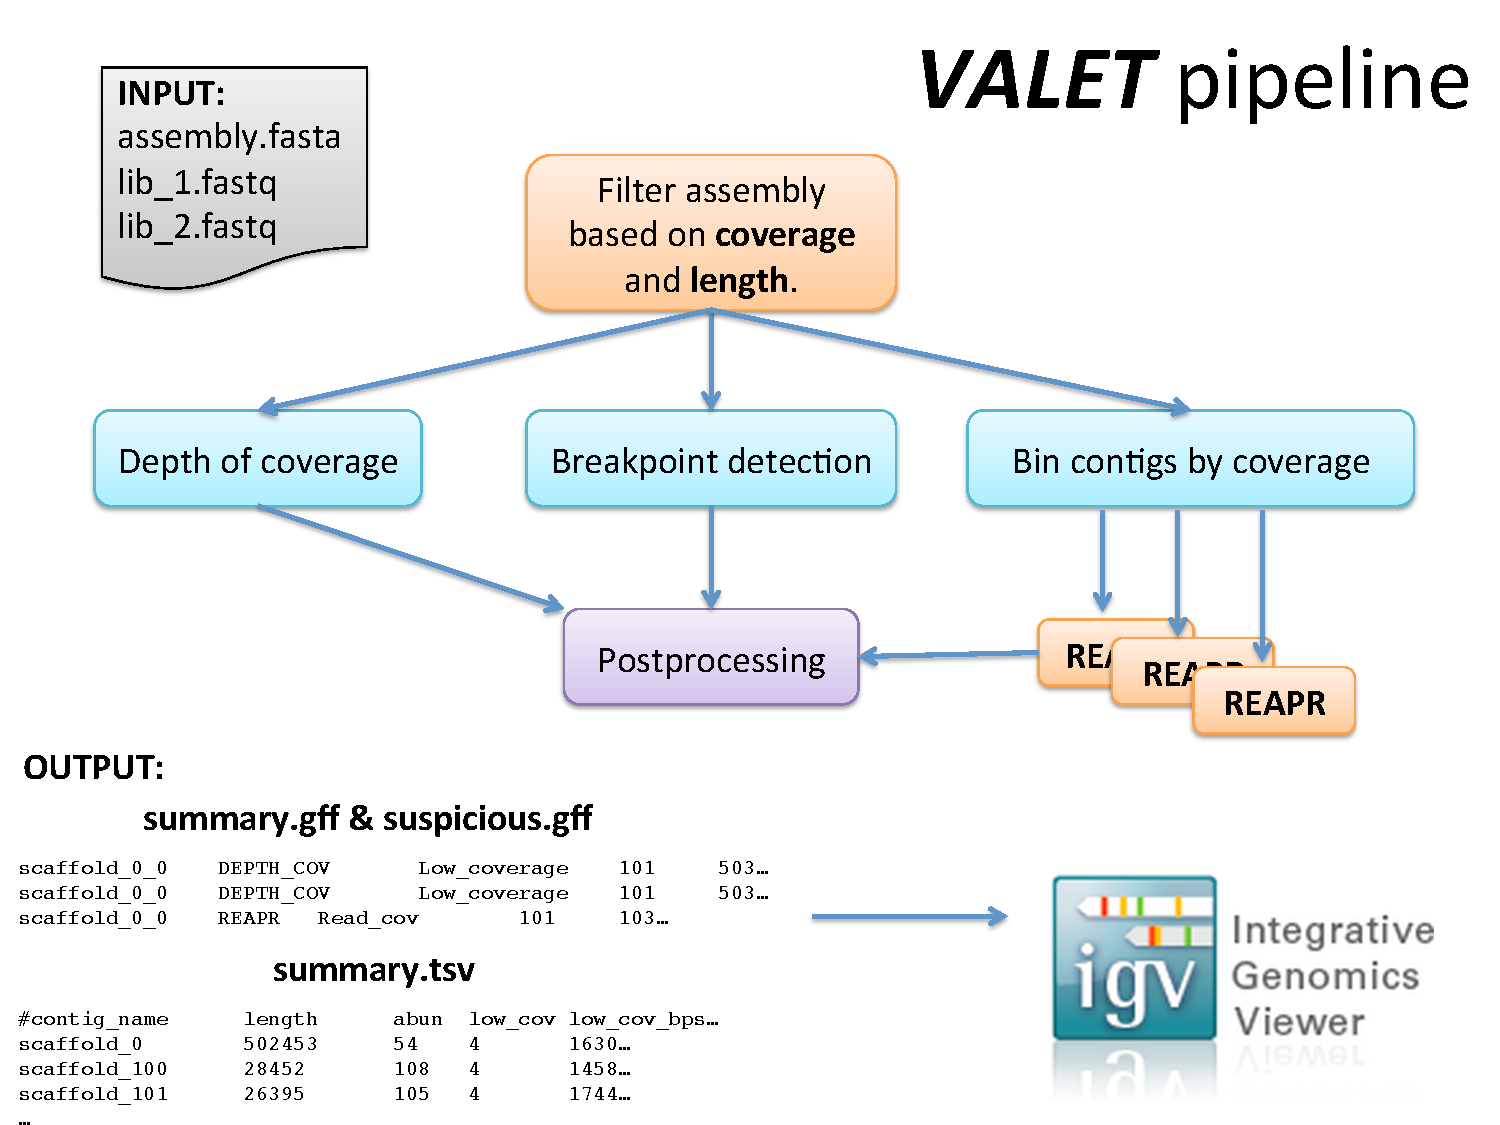
\includegraphics[width=3in]{figures/valet_pipeline}
\end{center}
\caption[valet_pipeline]{Digram of the VALET pipeline.}
%%%%%%%%%%%%%%%%%%%%%%%%% Need to add additional text
\label{fig:valet_pipeline}
\end{figure}

\begin{figure}[tb!]
\begin{center}
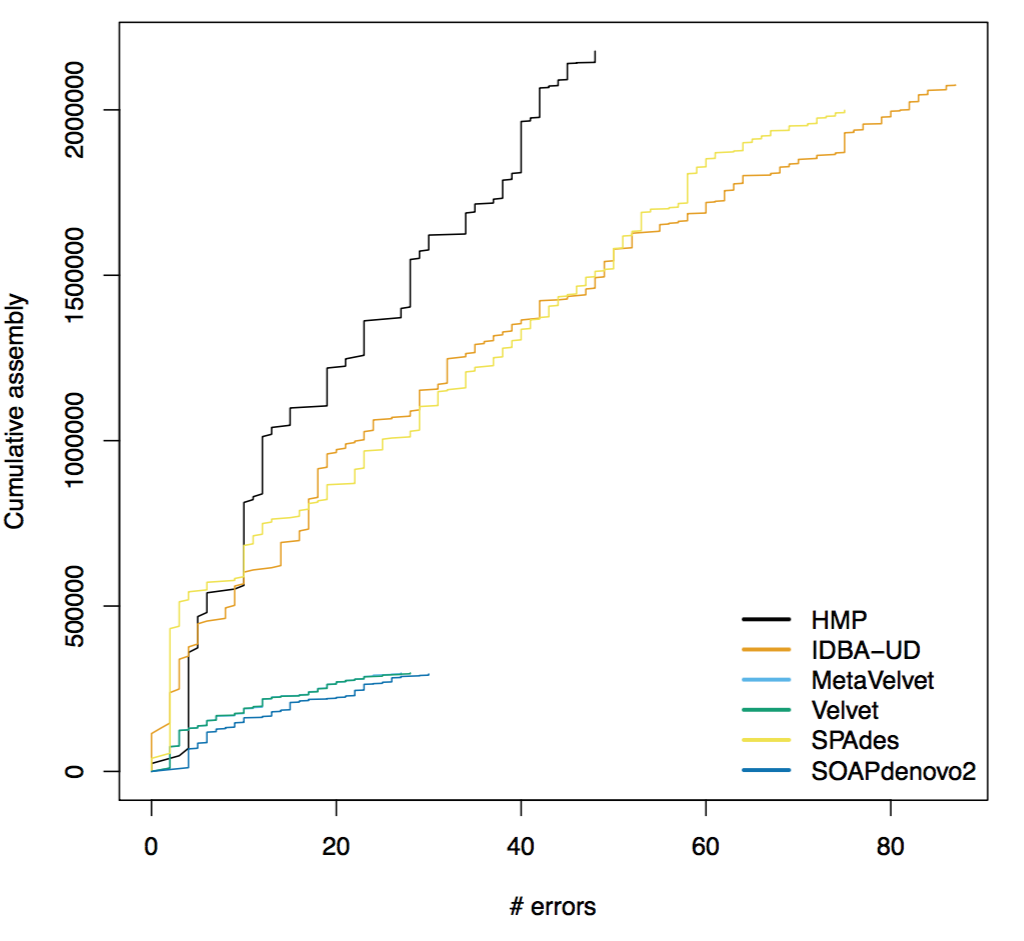
\includegraphics[width=3in]{figures/frc}
\end{center}
\caption[hmp_frc]{Feature Response Curve (FRC) plot produced by VALET comparing assemblies of a Vaginal introitus sample (SRS014465) from the Human Microbiome Project~\citep{human2012structure} (using IDBA-UD~\citep{peng2012idba}, MetaVelvet~\citep{namiki2012metavelvet}, Velvet~\citep{zerbino2008velvet}, SPAdes\citep{bankevich2012spades}, and SOAPdenovo2~\citep{luo2012soapdenovo2}. Point $(x,y)$ corresponds to the number of errors incurred, $y$, after processing the longest contigs until $x$ bp is reached.}
\label{fig:hmp_frc}
\end{figure}

\subsection{Comparing multiple assemblies}

We visualize the quality of an assembly by recording the number of errors accumulated as we add contigs in decreasing order of length using a Frequency Response Curve (FRC) plot __REF__.
This allows for quick visual comparison a set of metagenomic assemblies.


\subsection{VALET pipeline}

VALET takes as input a metagenome assembly \textsc{FASTA} file and a collection of paired and un-paired reads (Figure~\ref{fig:valet_pipeline}).
Assembled contigs are first filtered out based on size (2x the average read length by default).
Next the abundances of contigs are calculated by aligning the reads to the assembly with Bowtie 2~\citep{langmead2012fast} and samtools~\citep{li2009sequence}.
Contigs undergo an additional filtering step removing low abundance (i.e. coverage) contigs (10x by default).
Less data (sequencing reads) are available to detect mis-assemblies for lower coverage and shorter contigs. 
Therefore, higher coverage and longer sequence provide a better baseline for detecting mis-assemblies.

Once filtering has finished, regions of the assembly are flagged based on the inconsistencies described above.
In practice, most mis-assembly signatures have high false positive rates.
The false positive rate can be reduced by focusing on regions where multiple signatures agree.  
Therefore, any window of the assembly (2000 bp in length by default) that contains multiple mis-assembly signatures are marked as \textbf{suspicious}.
The flagged and suspicious regions are stored in a \textsc{BED} file, which allows users to visualize the mis-assemblies using any genomic viewers, such as \text{IGV}~\citep{thorvaldsdottir2012integrative}.
The excluding regions without multiple mis-assembly signatures may lead to additional false negatives. It is important for the user to be aware of the trade-off and use the filtered or unfiltered set of mis-assemblies that is more appropriate for their application.
%Regions that share multiple mis-assembly signatures may be more likely an \textit{actual} mis-assembly.


\begin{figure*}[tb!]
\begin{center}
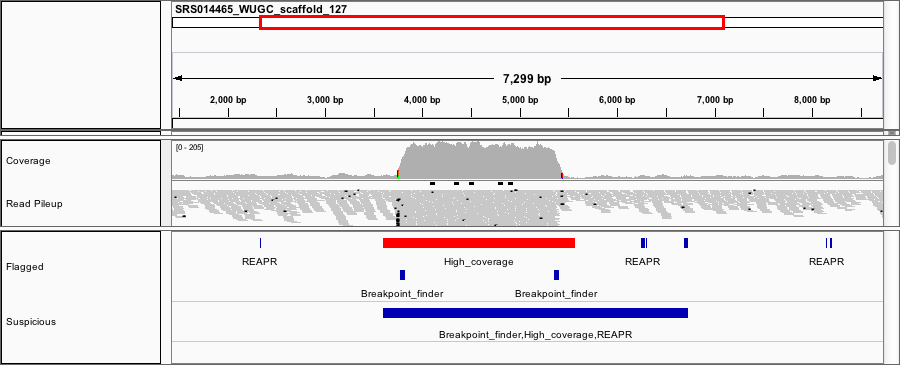
\includegraphics[width=.75\textwidth]{figures/hmp_plasmid}
\end{center}
\caption[hmp_plasmid]{An example suspicious region flagged by VALET in the HMP assembly of of a Vaginal introitus sample (SRS014465) from the Human Microbiome Project~\citep{human2012structure}.}
\label{fig:valet_igv}
\end{figure*}


\subsection{Using VALET to compare assemblies of a sample from the Human Microbiome Project}

Assemblies of a Vaginal introitus sample (SRS014465) from the Human Microbiome Project~\citep{human2012structure} (using IDBA-UD~\citep{peng2012idba}, MetaVelvet~\citep{namiki2012metavelvet}, Velvet~\citep{zerbino2008velvet}, SPAdes\citep{bankevich2012spades}, and SOAPdenovo2~\citep{luo2012soapdenovo2}.
Using VALET, we can compare the accumulated predicted error versus cumulative assembly length for each of the assemblies (Figure \ref{fig:hmp_frc}).
From this plot we can observe that the HMP assembly is accumulating errors at the lowest rate compared to the other assemblers.

The suspicious regions flagged by VALET combined with the IGV support provide researchers with a powerful starting point in their mis-assembly investigation.
For example, lets look at one of the suspicious regions flagged in the HMP assembly (Figure \ref{fig:valet_igv}.
VALET flags a 1.7 kbp high coverage region flanked by breakpoints.
This region BLASTs~\citep{BLAST} to \emph{Lactobacillus amylovorus} GRL 1118 plasmid2 (CP002611.1).
The right flanking region of the contig from positions 5,362 to 10,839 aligns to \emph{Lactobacillus crispatus} ST1, strain ST1 (FN692037.1) with 98\% similarity.
The left flanking ~3.75 kb region does not have a complete alignment with any sequence in NCBI; the closest alignment being from positions 1 to 2,599 to \emph{Lactobacillus helveticus} strain KLDS1.8701 (CP009907.1).
Researchers can now investigate further if this contig is mis-assemblies and composed of two closely-related species, or in fact, a novel species.

\section{Conclusion}

VALET is the first \emph{de novo} pipeline for detecting mis-assemblies in metagenomic datasets.
VALET allows researchers to find regions of their assemblies that are statistically inconsistent with characteristics of the sequence data generation process.


\section*{Acknowledgement}

\paragraph{Funding\textcolon} Text Text Text Text Text Text  Text Text.

\bibliographystyle{natbib}
% \bibliographystyle{achemnat}
% \bibliographystyle{plainnat}
% \bibliographystyle{abbrv}
% \bibliographystyle{bioinformatics}

\bibliographystyle{plain}

\bibliography{valet}

\end{document}
